\begin{observation}
	Consider the ring of integers $(\Z,+,\times)$. For $n\neq 1$, consider the set of integer multiplies $n\Z$.
	Then $1\notin n\Z$, but $(n\Z,\times)$ is closed under $\times$. That is, $n\Z$ is closed under $\times$ but not actually multiplicatively closed.
\end{observation}
\defbox[Multiplicatively Closed Subset of Ring]{\begin{definition}
	Let $(R,+,\times)$ be a ring with unity $1_S$ and zero $0_S$. Then $S\subseteq R$ is \textbf{multiplicatively closed} iff \begin{itemize}
		\item $1_R\in S$.
		\item $x,y\in S\implies x*y\in S$.
	\end{itemize}
\end{definition}}

\begin{note}[From $\Z$ to $\Q$]
\ \begin{itemize}
	\item (Numerator) $R=\Z$ is a ring
	\item (Denominators) $S=\Z\setminus\set{0}$ is multiplicatively closed and $1\in S$
	\item ($\Q\simeq S^{-1}R$) Every $q\in\Q$ is of the form $s^{-1}r$ for $r\in R$ and $s\in S$.
	\item (Equivalence Relation) \[
	\frac{a}{b}=\frac{c}{d}\iff ad=bc\iff t(ab-bc)=0\ \text{for}\ t\in S.
	\]
	\item $\Q$ is ring: \begin{itemize}
		\item $Q$ has an addition $a/b+c/d=(da+bc)/bd$
		\item $Q$ has a multiplication $a/b\cdot c/d=ac/bd$
		\item $Q$ has a zero $0/1$ and a one $1/1$.
	\end{itemize}
	\item $\Z$ is a subring of $\Q$ by $r\mapsto r/1$.
\end{itemize}
\end{note}

\begin{note}[Functions close to $0$ - "local functions"]
	\ \begin{itemize}
		\item (Numerator) $R=\R[x]\in\R^\R$ is a ring
		\item (Denominators) $S=\set{s\in R:s(0)\neq 0}$ is multiplicatively closed and $1\in S$
		\item ($L\simeq S^{-1}R$) Every local function $L$ is of the form $s^{-1}r$ for $r\in R$ and $s\in S$.
		\item (Equivalence Relation) \[
		\frac{a}{b}=\frac{c}{d}\iff ad=bc\iff t(ab-bc)=0\ \text{for}\ t\in S.
		\]
		\item Local function is ring: \begin{itemize}
			\item $L$ has an addition $a/b+c/d=(da+bc)/bd$
			\item $L$ has a multiplication $a/b\cdot c/d=ac/bd$
			\item $L$ has a zero $0/1$ and a one $1/1$.
		\end{itemize}
		\item $R$ has a map to $L$ by $r\mapsto r/1$.
	\end{itemize}
\end{note}

\section{For completeness: The formal definition/statement}
Let $R$ be a commutative ring and $S$ be a multiplicatively closed set with $1\in S$.
\begin{enumerate}[(a)]
	\item Equivalence Relation on $R\times S$ \[
	(a,b)\sim(c,d)\iff\exists t\in S:t(ad-bc)=0.
	\]
	\item \ [Localization (localize at $S$)] The set of equivalence classes $S^{-1}R$.
	\item Addition on $S^{-1}R$ \[
	(a,b)+(c,d)=(ad+bc, bd)
	\]
	\item Multiplication on $S^{-1}R$ \[
	(a,b)\cdot(c,d)=(ab,cd)
	\]
	\item (Slogan. Invert elements of $S$) \begin{itemize}
		\item $S^{-1}R$ is a ring with zero $(0,1)$ and one $(1,1)$
		\item There is a ring homomorphism $\phi:R\to S^{-1}R$ given by $r\mapsto (r,1),\ie, r\mapsto r/1$
		\item $\phi$ is injective ($R$ is a subring of $S^{-1}R$) iff $S$ contains no zero divisor
	\end{itemize}
\end{enumerate}

\begin{center}
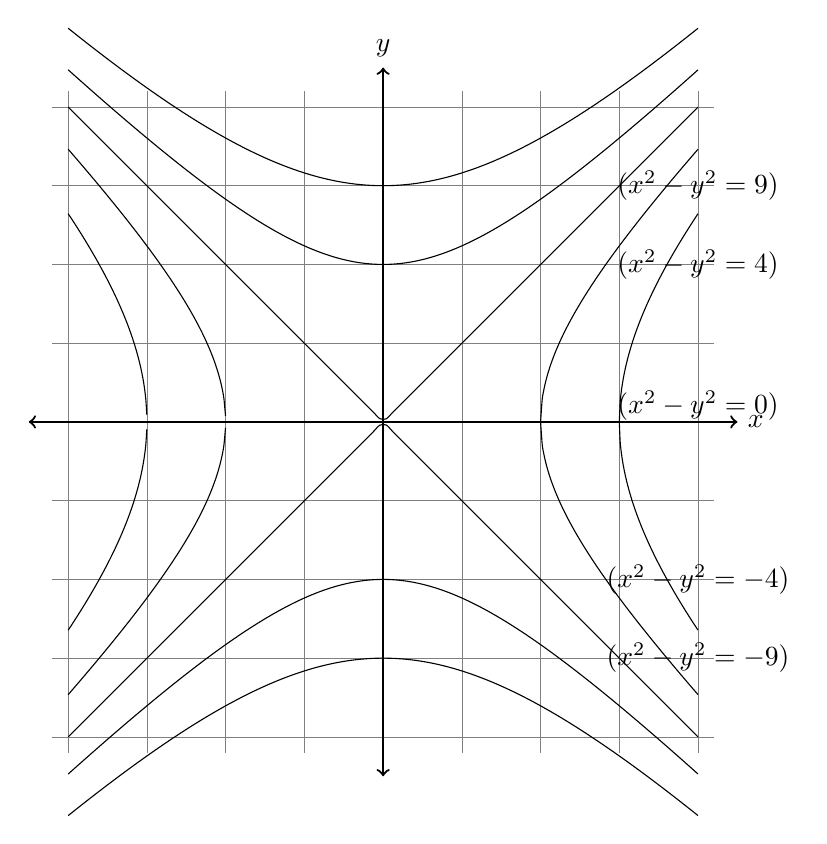
\begin{tikzpicture}
	% Axis settings
	\draw[very thin,color=gray] (-4.2,-4.2) grid (4.2,4.2);
	\draw[thick,<->] (-4.5,0) -- (4.5,0) node[right] {$x$};
	\draw[thick,<->] (0,-4.5) -- (0,4.5) node[above] {$y$};
	
	% Level curves for different values of k
	\foreach \k in {-9,-4,0,4,9} {
		% Plot the upper and lower branches of the hyperbolas
		\ifnum \k > 0
		\draw[domain=sqrt(\k):4, smooth, variable=\x, samples=100] 
		plot ({\x}, {sqrt(\x*\x - \k)});
		\draw[domain=sqrt(\k):4, smooth, variable=\x, samples=100] 
		plot ({\x}, {-sqrt(\x*\x - \k)});
		\draw[domain=-4:-sqrt(\k), smooth, variable=\x, samples=100] 
		plot ({\x}, {sqrt(\x*\x - \k)});
		\draw[domain=-4:-sqrt(\k), smooth, variable=\x, samples=100] 
		plot ({\x}, {-sqrt(\x*\x - \k)});
		\else
		\draw[domain=-4:4, smooth, variable=\x, samples=100] 
		plot ({\x}, {sqrt(\x*\x - \k)});
		\draw[domain=-4:4, smooth, variable=\x, samples=100] 
		plot ({\x}, {-sqrt(\x*\x - \k)});
		\fi
	}
	
	% Labels for the curves
	\node at (4,3) {$(x^2 - y^2 = 9)$};
	\node at (4,2) {$(x^2 - y^2 = 4)$};
	\node at (4,0.2) {$(x^2 - y^2 = 0)$};
	\node at (4,-2) {$(x^2 - y^2 = -4)$};
	\node at (4,-3) {$(x^2 - y^2 = -9)$};
\end{tikzpicture}
\end{center}

\begin{itemize}
	\item $X\subset\neq\R^2$ is the vanishing set of $(x-y)(x+y)$
	\item Model: the ring $R=\R[x,y]/\generate{(x-y)(x+y)}$
	\item $\generate{x-y}:X\to\R$ is locally at a indistinguishable from $0$
	\item $\generate{x-y}-0\neq 0$ but $(x+y)\generate{x-y-0}=0$ in $R$
	\item So $\generate{x-y}=0$ in $R$ localized at $S=\set{s\in R:s(a)=0}$.
\end{itemize}